\section{Neutrinos}

% █ What are neutrinos? What is neutrino astronomy?
Neutrinos are elementary particles with no electric charge and small mass. % [very] small mass…
Their low interactivity
  makes them difficult to detect,
  but is also the reason why they are valuable messenger particles for astroparticle physics:
Since they are not affected by the electromagnetic force,
% and very little by gravity,
  cosmic magnetic fields have no effect on their propagation paths \cite{neutrinos_katz};
  neither does the interstellar medium absorb them in significant amounts.
Together with the energy of the neutrino,
  the direction of propagation % / this information
  is used to determine the location and properties of the source \cite{neutrinos_katz}.


% █ Sources
Neutrinos have various astronomical sources,
  many of which are not experimentally confirmed yet.
This includes
  the \ac{CNB} \cite{follin2015}
     which originates from the Big Bang
  as well as various sources of cosmic ray acceleration
    (and therefore neutrino emission)
  \cite{neutrinos_aartsen_sources},
  such as
    \ac{SNR} shocks,
    \acp{AGN},
    jets,
    starburst galaxies, % Oxford comma
    and gamma-ray bursts.
Neutrinos are also produced in
  the Sun
  and in the Earth's atmosphere % due to cosmic rays!
  as well as in nuclear reactors.
They cover a vast range of energies, from \si{\micro\electronvolt} up to \si{\peta\electronvolt},
  depending on the source. % \citationneeded{}
\autoref{fig:neutrinos:flux_spectrum} shows the flux spectrum of neutrinos from different sources.

\begin{figure}
  \centering
  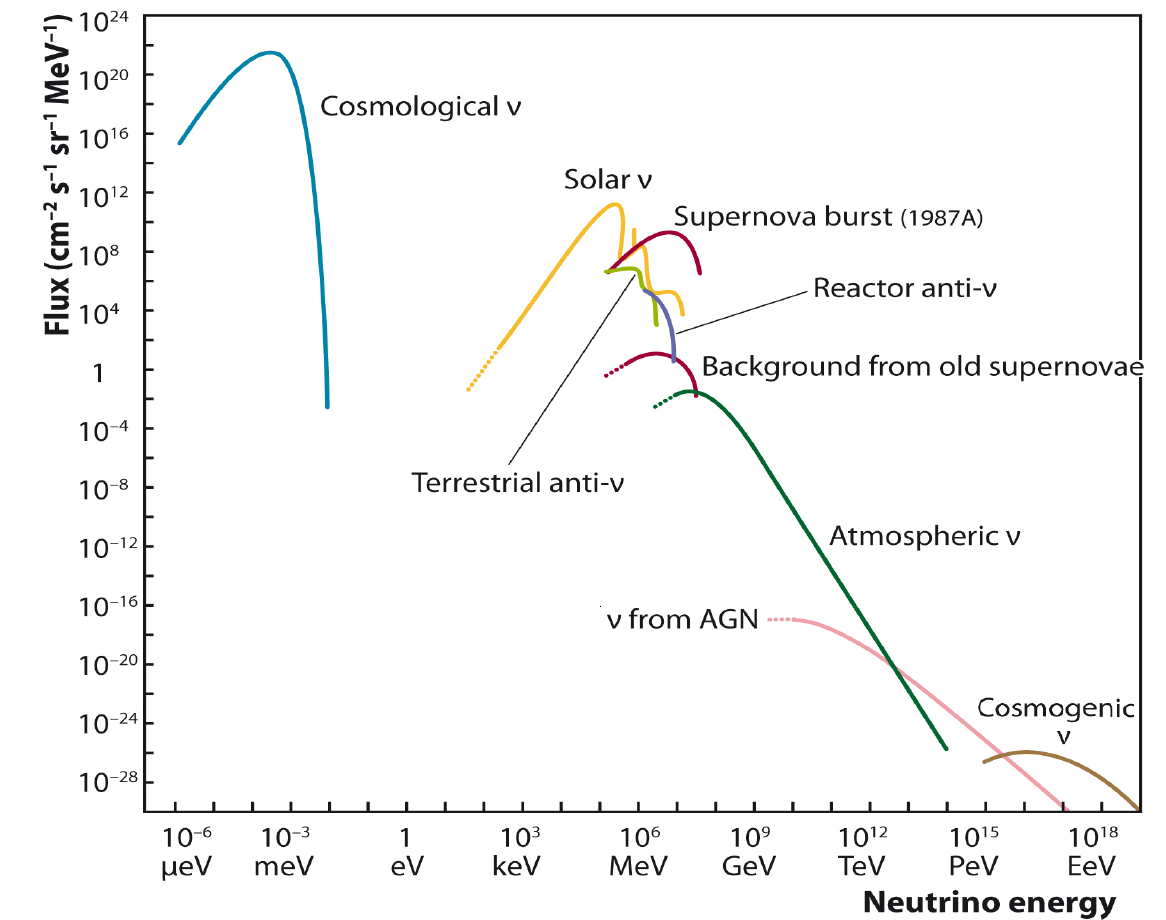
\includegraphics[width=0.75\textwidth]{content/img/neutrino_spectrum.png}
  \caption{
    Measured and expected fluxes of natural and reactor neutrinos as a function of their energy \cite{spiering2012}.
  }
  \label{fig:neutrinos:flux_spectrum}
\end{figure}


% █ Neutrino oscillations
While current models of astrophysical neutrino sources predict a flavor ratio of
  $\phi(\nu_e) : \phi(\nu_\mu) : \phi(\nu_\tau) = 1 : 2 : 0$
    (assuming charged pions decays are the dominant mechanism for neutrino production),
the observed ratio on Earth is
  $1 : 1 : 1$ \cite{neutrinos_beacom}.
This discrepancy is explained by neutrino oscillations \cite{neutrinos_beacom},
  which are a consequence of the fact that neutrinos have mass.
Albeit being very light
  (the current lowest upper limit on the Majorana mass being \qtyrange{0.06}{0.161}{\electronvolt} \cite{neutrinos_gando}),
  it allows for oscillations between the different flavors,
    given the large distances that cosmic neutrinos travel.
